%\documentclass[handout]{beamer}
\documentclass[compress]{beamer}

\usepackage[latin1]{inputenc}
\usepackage[english]{babel}
\usepackage{multimedia}

\usepackage{listings}
%\usepackage{times,mathptmx}
%\usepackage{palatino,mathpple}
\usepackage{pifont}
\usepackage{array}
\usepackage{graphicx,tikz,colortbl}
\usepackage{pgfpages}
\usetikzlibrary{arrows}

%%%%%%%%%%%%%%%%%%%%%%%%%%%%%%%%%%%%%%%%%%%%%%%%%%%%%%%%%%%%%%%%%%%%%%
\makeatletter
\errorcontextlines=5

\setlength{\overfullrule}{10pt}

\definecolor{mygreen}{RGB}{23, 120, 49}
\definecolor{darkgreen}{RGB}{50, 157, 76}
\definecolor{lightgreen}{RGB}{238, 255, 151}
\definecolor{umhblue}{RGB}{1, 56, 147}
\definecolor{thm title}{RGB}{172, 10, 45}
\definecolor{orangered}{RGB}{245, 94, 39}
\definecolor{mauve}{RGB}{179, 52, 77}

\definecolor{ocamlblue}{RGB}{102,102,255}
\definecolor{lightblue}{RGB}{190,199,254}
\definecolor{ocamlred}{RGB}{204,102,102}
\definecolor{ocamlred2}{RGB}{209, 78,78}
\definecolor{jsblue}{RGB}{32,70,148}

\mode<presentation|handout>{%
  \usetheme{Darmstadt}
  \useoutertheme[subsection=false]{miniframes}
%  \useinnertheme[shadow]{rounded}
  \setbeamercovered{transparent=5}
  \usecolortheme[named=ocamlblue]{structure}
  \setbeamercolor{block title}{bg=thm title,fg=yellow!15}
  \setbeamercolor{block body}{bg=ocamlred!10}
  \setbeamercolor{block title example}{bg=umhblue}
  \setbeamercolor{block body example}{bg=yellow!15}
  \setbeamercolor{alerted text}{fg=ocamlred2}
}

% \mode<presentation|handout:0> {%
%   \AtBeginDocument{%
%     \pgfdeclareverticalshading{beamer@headfade}{\paperwidth}
%     {%
%       color(0cm)=(bg);
%       color(1cm)=(umhblue!20)%
%      }
%   }
%   \addtoheadtemplate{\pgfuseshading{beamer@headfade}\vskip-1cm}{}
% }

\mode<handout>{
  \pgfpagesuselayout{4 on 1}[a4paper, border shrink=5mm,landscape]
}

\renewcommand{\>}{\ding{43}}
\renewcommand{\_}{\vrule height 0pt width 1ex depth 0.7pt}
\newcommand{\abs}[1]{\mathopen|#1\mathclose|}
\newcommand{\norm}[1]{\mathopen\|#1\mathclose\|}
\newcommand{\limplies}{\Rightarrow}
\newcommand{\bigdownarrow}[1]{%
  $\left\downarrow \vrule height#1 depth#1 width0pt\right.$%
  \hspace*{-0.2ex}\ignorespaces}

\renewcommand{\emph}[1]{%
  \textcolor{orangered}{#1}}

\newcommand{\ocamlfile}[2][]{%
  \begin{block}{}
    \vspace*{-1ex}%
    \lstinputlisting[language=caml,#1]{#2}%
    \vspace*{-1ex}%
  \end{block}}

\newenvironment{ocamlcode}{%
  \begin{block}{}
    \ttfamily
  }{%
  \end{block}
}

\newbox\underlinebox
\AtBeginDocument{%
\renewcommand{\underline}[2][black]{%
  \setbox\underlinebox=\hbox{#2}%
  \leavevmode
  \rlap{\raisebox{-2pt}{\color{#1}\rule{\wd\underlinebox}{0.8pt}}}%
  \box\underlinebox
}
}

\makeatother
%%%%%%%%%%%%%%%%%%%%%%%%%%%%%%%%%%%%%%%%%%%%%%%%%%%%%%%%%%%%%%%%%%%%%%

\pgfdeclareimage[width=8mm]{UMH-logo}{Acad-logoumh}
\pgfdeclareimage[width=8mm]{Acad-logo}{Acad-logo+txt}
\pgfdeclareimage[width=5mm]{ocaml}{caml05}

\title{Delimited overloading}
\author{Christophe Troestler}
\date[OCaml users meeting 2009]{\scriptsize %
  \textit{OCaml users meeting}\\
  February 4, 2009\\
  Grenoble\\
  \pgfuseimage{ocaml}}
\institute[UMH]{%
  Institut de Math�matique\\
  Universit� de Mons-Hainaut\\
  Mons, Belgium\\[5pt]
  \pgfuseimage{UMH-logo}\qquad
  \raisebox{-1mm}{\pgfuseimage{Acad-logo}}%
}
%\logo{\pgfuseimage{UMH-logo}}

\begin{document}

\lstset{language=Caml,basicstyle=\ttfamily}

\begin{frame}[plain]
  \titlepage
\end{frame}

\section*{Credits}
\begin{frame} \frametitle{Acknowledgments}
  This project was started thanks to the support of
  \raisebox{-1.1ex}{\colorbox{blue}{%
    
\includegraphics[width=0.3\linewidth]{jane-street-logo}}}
  who sponsored
  \vspace{1ex}
  \begin{itemize}
  \item
    \raisebox{-4ex}{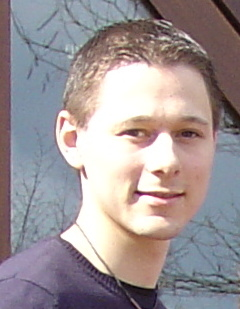
\includegraphics[width=0.12\linewidth]{Dany}}%
    \hspace{1em}%
    Dany Maslowski and
    \vspace{1ex}
  \item
    \raisebox{-4ex}{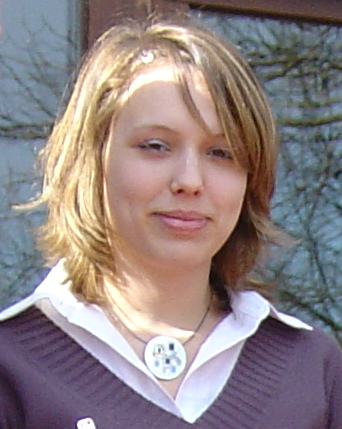
\includegraphics[width=0.12\linewidth]{Julie}}%
    \hspace{1em}%
    Julie De Pril
  \end{itemize}
  \vspace{1ex}
  during their OCaml summer projet 2008.
\end{frame}

\section*{Outline}
\begin{frame}\frametitle{Outline}
  \tableofcontents[subsectionstyle=hide]
\end{frame}

\section{Standard Overloadings}
\begin{frame}\frametitle{Outline}
  \tableofcontents[currentsection,subsectionstyle=hide]
\end{frame}

\begin{frame}\frametitle{Basic idea}
  \begin{center}
    \texttt{\LARGE M.(e) ${\mapsto}\  \sigma_{\mathtt{M}}$(e)}\\
    \vspace{3ex}%
    Operators,... in the expression \texttt{e} are overloaded
    according to the overloadings defined for the module name
    \texttt{M}.
  \end{center}
\end{frame}

\begin{frame}\frametitle{Basic use}

  \begin{ocamlcode}
    Float.(\alert<1>{1 +} x \alert<1>{*} f \alert<1>{4})\\
    Float.(\alert<1>{4 *} u**\alert<1>{2 /} sqrt(\alert<1>{abs} alpha))\\
    %Hashtbl.(\alert<1>{h.(key)})\\
    Hashtbl.(h\alert<1>{.(}key\alert<1>{) <-} x)
  \end{ocamlcode}
  \> Literals, functions, and ``constant constructions'' substitution.\\
  \> Better readability.

  \onslide<2->%
  \vspace{2ex}

  \begin{ocamlcode}
    Big\_int.(\textbf{if} x \alert<2>{>} 0 \textbf{then} 1 + x \textbf{else} 0)
  \end{ocamlcode}
  \> Can use the usual comparison operators.

  \onslide<3->%
  \vspace{2ex}
  \begin{ocamlcode}
    \alert<3>{Int32.(}4 + a.(\alert<3>{Int.(}1 + x\alert<3>{)})\alert<3>{)}
  \end{ocamlcode}
  \> Nested overloadings.
\end{frame}

\begin{frame}\frametitle{Static checks \& simple optimizations}

  \begin{ocamlcode}
    Num.(\alert<1>{"12345678"} + x)
  \end{ocamlcode}
  \> Compile time check.\\
  If one writes \texttt{Num.("a12")}, when compiling, the following
  error is issued\\
  \begin{alertblock}{}
    \texttt{Parse error: The string "a12" does not represent a valid Num.\\
      Preprocessing error on file foo.ml}
  \end{alertblock}

  \onslide<2->%
  \vspace{1ex}
  \begin{ocamlcode}
    Float.(\alert<2>{(x+1)**2})
  \end{ocamlcode}

  \> Simple optimization.   The whole expression is substituted by
  (binding introduced only if needed):\\
  \centerline{\texttt{let \textit{tmp} = x +.\ 1.0 in \textit{tmp} *.\
      \textit{tmp}}}
\end{frame}

\begin{frame}\frametitle{Complex numbers}
  \begin{ocamlcode}
    Complex.({\textbf{let}} z = 3 + 2 \alert<1>{I} {\textbf{in}}
    \alert<1>{sin}(z * z))
  \end{ocamlcode}
  \> ``\texttt{I}'' notation.\\
  \> Let binding are allowed.\\
  \> Complex functions like \texttt{sin}, \texttt{cos},...
  are inlined.\note{inlined... when it makes sense}

  \onslide<2->%
  For example,
  \begin{ocamlcode}
    \small{Complex.((2 + 3 I) * f x)}
  \end{ocamlcode}
  is turned into
  \begin{ocamlcode}
    \textbf{let} \textit{tmp} = f x \textbf{in}\\
    \{ Complex.re = (\textit{tmp}.Complex.re *.\hspace{-0.6em} 2.0) -.
    \hspace*{10em}(\textit{tmp}.Complex.im *.\hspace{-0.6em} 3.0);\\
    \ \ Complex.im = (\textit{tmp}.Complex.re *.\hspace{-0.6em} 3.0) +.
    \hspace*{10em}(\textit{tmp}.Complex.im *.\hspace{-0.6em} 2.0);     \}
  \end{ocamlcode}
\end{frame}

\begin{frame}\frametitle{Summary}

  \colorbox{lightblue}{\texttt{pa\_do.cmo}} provides
  overloadings for
  \begin{center}
    \begin{tabular}{lll}
      \texttt{Int}& 	\texttt{Float}& 	\texttt{Hashtbl}\\
      \texttt{Int32}&	\texttt{Complex}&	\texttt{String}\\
      \texttt{Int64}\\
      \texttt{Nativeint}
    \end{tabular}
  \end{center}

  \bigbreak
  \onslide<2>%
  \colorbox{lightblue}{\texttt{pa\_do\_nums.cmo}} provides
  overloadings for
  \begin{center}
    \begin{tabular}{l}
      \texttt{Num}\\
      \texttt{Ratio}\\
      \texttt{Big\_int}
    \end{tabular}
  \end{center}
  \> Requires \emph{\texttt{nums.cmo}} to be loaded by camlp4 for static
  checks.
\end{frame}


\section{Defining overloadings}
\begin{frame}\frametitle{Outline}
  \tableofcontents[currentsection,subsectionstyle=hide]
\end{frame}

\begin{frame}\frametitle{Concrete syntax v.s.\ API}
  \begin{center}
    \begin{tabular}{>{\columncolor{yellow!15}}p{4.83cm}|p{4.83cm}}
      \multicolumn{1}{>{\columncolor{yellow!15}}c|}{\textbf{Concrete syntax}}&
      \multicolumn{1}{c}{\textbf{API}}\\
      \hline \hline
      In the source file & In a separate file\\ \hline
      Must be repeated in each file & Can be bundled with a library\\ \hline
      \sloppy
      No possibility of  overloading general expressions &
      \sloppy
      One can overload general ex\-pres\-sions and perform some
      optimizations \\
      \hline
      \multicolumn{1}{c}{}&\multicolumn{1}{c}{\onslide<2>{%
          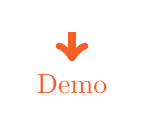
\begin{tikzpicture}[y=2.5ex]
            \draw[line width=3pt,->,color=orangered]
            (0,1) -- (0,0) node[below]{Demo};
          \end{tikzpicture}
        }}
    \end{tabular}
  \end{center}
\end{frame}

\begin{frame}\frametitle{``Set of overloadings''}

  \begin{center}
    \textbf{Constructions that can be overloaded:}\\
    literals\\
    \texttt{`x}\\
    \texttt{a.(i)}\\
    \texttt{a.(i) <- x}\\
    \texttt{a.[i]}\\
    \texttt{a.[i] <- x}\\
    \texttt{a.\{i\}}\\
    \texttt{a.\{i\} <- x}\\
    \texttt{a := x}\\
    \texttt{a <- x}\\
    \texttt{a.p}\\
    functions \& operators overloadings\\
    general substitutions
  \end{center}
\end{frame}

\begin{frame}\frametitle{How to overload one's own module (1/2)}
  \begin{ocamlcode}
    module Foo :\\
    sig\\
    \ \ type t\\
    \ \ val \alert<2>{of\_int} : int -> t\\
    \ \ val \alert<3>{compare} : t -> t -> int\\
    \ \ val \alert<4>{add} : t -> t -> t\\
    \ \ val \alert<4>{mul} : t -> t -> t\\
    end\\
  \end{ocamlcode}

  \onslide<2->%
  Overloading with the concrete syntax:
  \begin{itemize}
  \item<2-> int literals:
    \texttt{OVERLOAD\_INT Foo (\alert<2>{of\_int})}
  \item<3-> comparison:
    \texttt{OVERLOAD\_COMPARISON Foo (\alert<3>{compare})}
  \item<4-> functions:\\ \qquad
    \texttt{OVERLOAD Foo ( ( + ) -> \alert<4>{add}; ( * ) ->
      \alert<4>{mul} )}
  \end{itemize}
\end{frame}

\begin{frame}\frametitle{How to overload one's own module (2/2)}
  \textbf{Remarks}
  \vspace{2ex}
  \begin{itemize}[<+->]
  \item If \texttt{Foo} implements all standard functions
    \texttt{add}, \texttt{sub}, \texttt{mul}, \texttt{div} and
    \texttt{neg} (unary negation):\\
    \> \texttt{OVERLOAD\_ARITHMETIC Foo}.
    \vspace{2ex}
  \item<2-> If a new module is implemented:\\
    \begin{ocamlcode}
    module Special\_foo :\\
    sig\\
    \ \ include Foo\\
    \ \ val sub : t -> t -> t\\
    end\\
    \end{ocamlcode}
    \> \texttt{OVERLOAD Special\_foo \alert{inherit} Foo}\\
    \> \texttt{OVERLOAD Special\_foo ( ( - ) -> sub )}
  \end{itemize}
\end{frame}

\begin{frame} \frametitle{Some more examples}

  Basin of attraction of Newton's method for $z^3 = 1$.
  \begin{ocamlcode}
    Complex.(\\
    \ \  let z = ref z0 in\\
    \ \  for i = Int.(1) to niter do\\
    \ \ \ \  z := (\alert<1>{2 *} !z \alert<1>{+ 1 /} !z\alert<1>{**2})
    \alert<1>{/ 3}\\
    \ \  done;\\
    \ \  if \alert<1>{abs}(!z \alert<1>{-} root0) \alert<1>{<=} r
    then Some color0\\
%     \ \  else if abs(!z - root1) <= r then Some color1\\
%     \ \  else if abs(!z - root2) <= r then Some color2\\
%     \ \  else None\\
    \ \ $\ldots$
    )
  \end{ocamlcode}

  \onslide<2>\medbreak %
  Let $D = 1.7$. If $p = [p_0; \dotsc; p_n]$ represents the polynomial
  $\sum_{i=0}^{n} p_i z^i$, its norm is (here) defined by
  \begin{math}
    \norm{p} := \sum_{i=0}^n \abs{p_i} D^i
  \end{math}

  \begin{ocamlcode}
    let domain = Interval.(\alert<2>{17 / 10})\\
    let norm p = Interval.(List.fold\_right (fun c n ->\\
    \leavevmode\hfill
    \alert<2>{abs} c \alert<2>{+} domain \alert<2>{*} n) p \alert<2>{0})
  \end{ocamlcode}
\end{frame}


\section{Priority \& associativity}
\begin{frame}\frametitle{Outline}
  \tableofcontents[currentsection,subsectionstyle=hide]
\end{frame}
\begin{frame} \frametitle{Priority and associativity of operators}

  \colorbox{lightblue}{\texttt{pa\_infix.cmo}}

  \medbreak %
  Concrete syntax:
  \begin{ocamlcode}
    INFIX ( \%+ ) RIGHTA HIGHER (+)\\
    INFIX ( \^{}* ) LEVEL (+)\\
    PREFIX ( /+/ )\\
    POSTFIX ( /// ) LEVEL ( !\hspace{-1ex} )\\
  \end{ocamlcode}

  \medbreak %
  API: treat \texttt{a = b |> c} as \texttt{a = (b |> c)} and replace
  \texttt{x |> f} by \texttt{f x}:
  \par\vspace{-1ex}%
  \begin{ocamlcode}
    \small
    open Pa\_infix\\
    module L = Level\\
    let l = L.binary (L.Higher L.comparison) $\sim$assoc:L.LeftA in\\
    let expr x y \_loc = <:expr< \$y\$ \$x\$ >> in\\
    infix "|>" $\sim$expr l
  \end{ocamlcode}
\end{frame}


\section{Macros}
\begin{frame}\frametitle{Outline}
  \tableofcontents[currentsection,subsectionstyle=hide]
\end{frame}

\begin{frame} \frametitle{Collaboration with Delimited Overloading}

  \begin{ocamlcode}
    DEFINE NEWTON(M,x) = M.( (2 * x + 1 / x**2) / 3 )
  \end{ocamlcode}
  Use it as
  \begin{ocamlcode}
    NEWTON(Float, r)\\
    NEWTON(Complex, z)
  \end{ocamlcode}

  \> Poor man defunctorizer;\\
  \> Contrarily to functors, requalifies constants.
  \note{e.g. algorithm for floats and complex}

  % - API => other syntax extensions can be macro-aware
\end{frame}

\begin{frame} \frametitle{Better error reporting}

  \begin{ocamlcode}
    DEFINE A(x) =\\
    \ \ let s = ref 0.0 in\\
    \ \ for i = 1 to x do\\
    \ \ \ \ s :=
    \only<1>{!s}%
    \only<2->{\underline[darkgreen]{!s}}
    + float i\\
    \ \ done;\\
    \ \ s\\
    \ \\
    let () = print\_float(\underline[ocamlred]{A(100)})
  \end{ocamlcode}
  \only<1>{%
    \vtop to 20ex{%
      With the standard macros:
      \vspace{-1ex}%
      \begin{ocamlcode}
        \small
        \underline[ocamlred]{File "...", line 8, characters 21-27:}\\
        This expression has type float but is here used with type int
      \end{ocamlcode}
      \vss}}%
  \only<2->{%
    \vtop to 20ex{%
      With Delimited Overloading macros:
      \vspace{-1ex}%
      \begin{ocamlcode}
        \small
        \underline[ocamlred]{File "...", line 8, characters 21-27:}\\
        Expanding of the macro "A" at the previous location yields the error:\\
        \underline[darkgreen]{File "...", line 4, characters 11-13:}\\
        This expression has type float but is here used with type int
      \end{ocamlcode}
    \vss}}
\end{frame}


% \begin{frame} \frametitle{Other syntax extensions \& tests}

%   \textbf{Pa\_infix:} enable to set any OCaml operator as infix,
%   prefix or postfix and set its precedence and associativity.

%   \onslide<2->%
%   \vspace{3ex}%
%   \textbf{Test:} automatic and hierarchical testing framework for
%   syntax
%   extensions:\\
%   \> tests AST equality and computational equivalence (``behavioral''
%   testing);  randomly generated tests.

% \end{frame}



\section{Some technical details}
\begin{frame}\frametitle{Outline}
  \tableofcontents[currentsection]
\end{frame}

\subsection{Optimization for complex operators}
\begin{frame}\frametitle{Optimization for complex operators}
  \begin{ocamlcode}
    \small{Complex.((2 + 3 I) * f x)}
  \end{ocamlcode}

  \begin{enumerate}
  \item Classify subexpressions according to
    \begin{minipage}{0.7\linewidth}
      \begin{ocamlcode}
        type t =\\
        \ \ | Zero\\
        \ \ | Re of Ast.expr\\
        \ \ | Im of Ast.expr\\
        \ \ | Cplx of Ast.expr * Ast.expr\\
        \ \ | Unknown of Ast.expr
      \end{ocamlcode}
    \end{minipage}
\item Specialize complex functions, introducing bindings as needed.
  \end{enumerate}
\end{frame}

\subsection{Nested overloading}
\begin{frame}\frametitle{Nested overloading (1/3)}

  \begin{center}
    \texttt{M.(e) ${\mapsto}\  \sigma_{\mathtt{M}}$(e)}\\
    \vspace{1ex}
    where $\sigma_{\mathtt{M}} : expression \to expression$
  \end{center}
  \onslide<2->%
  \textbf{Problem encountered:}\\
  \begin{center}
    \texttt{Int32.(\alert<3>{a.(\alert<4>{Int.(0)}) <- 7 + x})}\\[1\jot]
    \onslide<4->%
    \textcolor{mauve}{%
      \bigdownarrow{1ex}%
      \rlap{apply $\sigma_{\mathtt{Int}}$;\ \
        here \texttt{$\sigma_{\mathtt{Int}}$(0) = 0}}}\\[1\jot]
    \onslide<5->%
    \texttt{Int32.(\alert<6>{a.(\alert<5>{0}) <- 7 + x})}\\[1\jot]
    \onslide<6->%
    \textcolor{mauve}{\bigdownarrow{1ex}%
      \rlap{apply $\sigma_{\mathtt{Int32}}$}}\\[1\jot]
    \onslide<7->%
    \texttt{a.(\textcolor<8->{red}{0l}) <- Int32.add 7l x}\\[1.5ex]
    \onslide<8->%
    \textcolor{red}{Problem!}
  \end{center}
  \onslide<9->%
  \> Protection of already overloaded expressions
\end{frame}

\begin{frame}\frametitle{Nested overloading (2/3)}

  \textbf{Requirements:}
  \begin{itemize}[<+->]
  \item \texttt{$\sigma_{\mathtt{Int}}$(0)} must be a valid expression;
  \item it must not change the meaning of the program nor its performance;
  \item locations  must not be affected (for correct error reporting).
  \end{itemize}
  \vspace{2ex}
  \onslide<4->%
  \textbf{Solution:}
  \begin{center}
    \texttt{M.(e) ${\mapsto}\
      \mathtt{\alert{p}}(\sigma_{\mathtt{M}}\mathtt{(e)})$}\\[1ex]
    where \alert{\texttt{p}} is an undeclared function name!
  \end{center}

  \tiny %
  \> \texttt{p} is removed by the surrounding overloading $\limplies$
  global flag to know whether to insert~$\pi$.
  \\[0.3ex]
  \> \textbf{external}\ $\texttt{p} : \alpha \to \alpha$ =
  \texttt{"\%identity"} forbid some optimizations to take place!
  \par
\end{frame}

\begin{frame}\frametitle{Nested overloading (3/3)}

  \begin{center}
    \texttt{Int32.(\alert<2>{a.(\alert<3>{Int.(0)}) <- 7 + x})}\\[1\jot]
    \onslide<3->%
    \textcolor{mauve}{\hspace{13.5em}%
      \bigdownarrow{1.5ex}
        \texttt{Int.(0) =
          $\texttt{p}(\sigma_{\mathtt{Int}}\mathtt{(0)})$
          = $\texttt{p}(0)$}}\\[1\jot]
    \onslide<4->%
    \texttt{Int32.(\alert<5>{a.(\alert<4,6>{$\texttt{p}$(0)}) <- 7 + x})}%
    \\[1\jot]
    \onslide<5->%
    \textcolor{mauve}{\hspace{-5em}%
      \bigdownarrow{1.5ex} apply $\sigma_{\mathtt{Int32}}$}\\[1\jot]
    \onslide<6->%
    \texttt{p(a.(\alert<6->{0}) <- Int32.add 7l x)}\\[2ex]
    \onslide<7->%
    \textcolor{red}{OK!}
  \end{center}
\end{frame}

\subsection{General substitution of expressions}
\begin{frame}\frametitle{General substitution of expressions \texttt{M.($e$)}}
  \begin{center}
    \begin{tikzpicture}[x=1ex,y=1ex,>=stealth']
      \tikzstyle{state}=[draw,rectangle,text centered]
      \node (self) at (0,16) {};
      \node[state] (pi) at (0,15) {$\pi$};

      \node[state] (BO) at (0,-10) {\small{basic overloadings}};
      \node[state] (map) at (0,-16) {\texttt{Ast.map\#expr}};

      \node (se) at (22,0) {\small{Substituted expression}};
      \node (oe) at (-20,20) {\small{Original expression $e$}};

      \onslide<4->{%
        \node[state] (f1) at (0,-5) {$\mathtt{f_1}$};
        \draw[thick,->,color=orangered] (f1) -- (BO)
        node[right,pos=0.5,color=orangered,font=\footnotesize]{%
          \texttt{super}};
        \only<4->{%
          \draw[thick,->,color=darkgreen] (f1)..controls(-9,-5)..(-9,0)..
          controls(-9,19)..(self);}
        \draw[thick,->] (f1)..controls(11,-5)..(se);
        \node[color=darkgreen,font=\footnotesize] at (-6.3,-3){\texttt{self}};
      }
      \onslide<5->{%
        \node[state] (f2) at (0,0) {$\mathtt{f_2}$};
        \draw[thick,->,color=orangered] (f2) -- (f1)
        node[right,pos=0.5,color=orangered,font=\footnotesize]{%
          \texttt{super}};
        \only<5->{%
          \draw[thick,->,color=darkgreen]
          (f2)..controls(-7,0)..(-7,3)..controls(-7,18.5)..(self);}
        \draw[thick,->] (f2)..controls(9,3)..(se);
        \node[font=\footnotesize,color=darkgreen] () at (-4.5,2) {%
          \texttt{self}};
      }
      \onslide<6->{%
        \begin{scope}[font=\footnotesize]
          \node[state] (fn) at (0,10) {$\mathtt{f_n}$};
          \draw[thick,->] (pi) -- (fn);
          \draw[thick,->,color=orangered] (fn) -- (0,6)
          node[right,pos=0.5,color=orangered]{\texttt{super}};
          \draw[thick,dashed,color=orangered] (0,6) -- (0,3.5);
          \draw[thick,->,color=orangered] (0,3.5) -- (f2)
          node[right,pos=0.5,color=orangered]{\texttt{super}};
          \only<6->{%
            \draw[thick,->,color=darkgreen]
            (fn)..controls(-5.5,10)..(-5.5,13)..controls(-5.5,18)..(self);}
          \draw[thick,->] (fn)..controls(8,9)..(se);
          \draw[thick,->] (pi) -- (fn);
          \node[color=darkgreen] () at (-3,12.5){\texttt{self}};
        \end{scope}
      }
      \only<1-3>{\draw[thick,->] (pi) -- (BO);}
      \only<4>{\draw[thick,->] (pi) -- (f1);}
      \only<5>{\draw[thick,->] (pi) -- (f2);}

      \onslide<2->{%
        \draw[thick,->,color=orangered] (BO) -- (map)
        node[right=0.5cm,above=0.25cm,color=orangered,font=\footnotesize]{%
          \texttt{super}};
      }
      \only<1>{\draw[thick,->] (BO) -- (map)};

      \draw[thick] (oe) -- (0,20);
      \draw[thick,->] (0,20) -- (pi);

      \only<3->{%
        \begin{scope}[color=darkgreen,font=\footnotesize]
          \draw[thick,->] (BO)..controls(-13,-10).. (-13,0)
          ..controls(-13,18) and (-11,20).. (self);
          \draw[thick,->] (map)..controls(-15,-15).. (-15,0)
          ..controls(-15,18) and (-11,20).. (self);
          \node at (-10.3,-7.5) {\texttt{self}};
          \node at (-11.3,-13) {\texttt{self}};
        \end{scope}
      }

      \draw[thick,->] (pi)..controls(12,12)..(se);
      \draw[thick,->] (BO)..controls(11,-10)..(se);
      \draw[thick,->] (map)..controls(13,-15)..(se);
    \end{tikzpicture}
  \end{center}
\end{frame}

\begin{frame}
  \begin{center}
    {\LARGE Thank you for your attention...}

    \vspace{3ex}
    and to Sylvain Le Gall, Alan Schmitt, and Serge Leblanc for
    organizing this meeting.
  \end{center}
\end{frame}



\end{document}
%%% Local Variables:
%%% mode: latex
%%% TeX-master: t
%%% TeX-PDF-mode: t
%%% End:
